\documentclass[twoside]{article}
\usepackage[a4paper]{geometry}
\geometry{verbose,tmargin=2.5cm,bmargin=2cm,lmargin=2cm,rmargin=2cm}
\usepackage{fancyhdr}
\pagestyle{fancy}

% nastavení pisma a~češtiny
\usepackage{lmodern}
\usepackage[T1]{fontenc}
\usepackage[utf8]{inputenc}
\usepackage[czech]{babel}

% odkazy
\usepackage{url}

\usepackage{float}
% vícesloupcové tabulky
\usepackage{multirow}
\usepackage{listings}
\usepackage{xcolor}
\usepackage{amssymb}
\usepackage{gensymb}
\usepackage{bbold}
\usepackage{amsmath}
\usepackage{siunitx}
\usepackage{mathtools}
\usepackage{commath}

% vnořené popisky obrázků
\usepackage{subcaption}

% automatická konverze EPS 
\usepackage{graphicx} 
\usepackage{epstopdf}
\epstopdfsetup{update}

\graphicspath{{./images}}

% odkazy a~záložky
\usepackage[unicode=true, bookmarks=true,bookmarksnumbered=true,
bookmarksopen=false, breaklinks=false,pdfborder={0 0 0},
pdfpagemode=UseNone,backref=false,colorlinks=true] {hyperref}


% Poznámky při překladu
\usepackage{xkeyval}	% Inline todonotes
\usepackage[textsize = footnotesize]{todonotes}
\presetkeys{todonotes}{inline}{}

%https://tex.stackexchange.com/questions/2783/bold-calligraphic-typeface
\DeclareMathAlphabet\mathbfcal{OMS}{cmsy}{b}{n}

% enumerate zacina s pismenem
\renewcommand{\theenumi}{\alph{enumi}}

% smaz aktualni page layout
\fancyhf{}
% zahlavi
\usepackage{titling}
\fancyhf[HC]{\thetitle}
\fancyhf[HLE,HRO]{\theauthor}
\fancyhf[HRE,HLO]{\today}
 %zapati
\fancyhf[FLE,FRO]{\thepage}

% údaje o autorovi
\title{OTE Domácí úkol 7a - Operační usměrňovač}
\author{Vojtěch Michal}
\date{\today}

%customize code listing
\definecolor{codegreen}{rgb}{0,0.6,0}
\definecolor{codegray}{rgb}{0.5,0.5,0.5}
\definecolor{codepurple}{rgb}{0.58,0,0.82}
\definecolor{backcolour}{rgb}{0.95,0.95,0.92}

\lstdefinestyle{mystyle}{
    backgroundcolor=\color{backcolour},   
    commentstyle=\color{codegreen},
    keywordstyle=\color{magenta},
    numberstyle=\tiny\color{codegray},
    stringstyle=\color{codepurple},
    basicstyle=\ttfamily\footnotesize,
    breakatwhitespace=false,         
    breaklines=true,                 
    captionpos=b,                    
    keepspaces=true,                 
    numbers=left,                    
    numbersep=5pt,                  
    showspaces=false,                
    showstringspaces=false,
    showtabs=false,                  
    tabsize=2
}

\lstset{style=mystyle}

\begin{document}

\maketitle

V simulacích pro tuto úlohu bylo použito nastavení parametrů operačního zesilovače uvedené v tabulce \ref{tab:oz_param}.

\begin{table}[h!]
    \centering
    \begin{tabular}{c|c|c|c|c}
        parametr & symbol & hodnota & jednotka & poznámka\\
        \hline
        Vstupní napěťový offset & $U_0$ & 1 & \si{\milli\volt} & \\
        Vstupní klidový proud & $I_\text{B}$ & 50 & \si{\nano\ampere} & $(I_\text{BP} + I_\text{BN})/2$ \\
        Vstupní zbytkový proud & $I_0$ & 20 & \si{\nano\ampere} & $I_\text{BP} - I_\text{BN}$ \\
        Zesílení v otevřené smyčce & $A_\text{D}$ & 200 & \si{\kilo\volt\per\volt} & \\
        Tranzitní kmitočet& $f_T$ & 1 & \si{\mega\hertz} &
    \end{tabular}
    \caption{Parametry operačního zesilovače použité pro simulaci}
    \label{tab:oz_param}
\end{table}

\section{Ověření funkce obvodu}

\begin{figure}[h!]
    \centering
    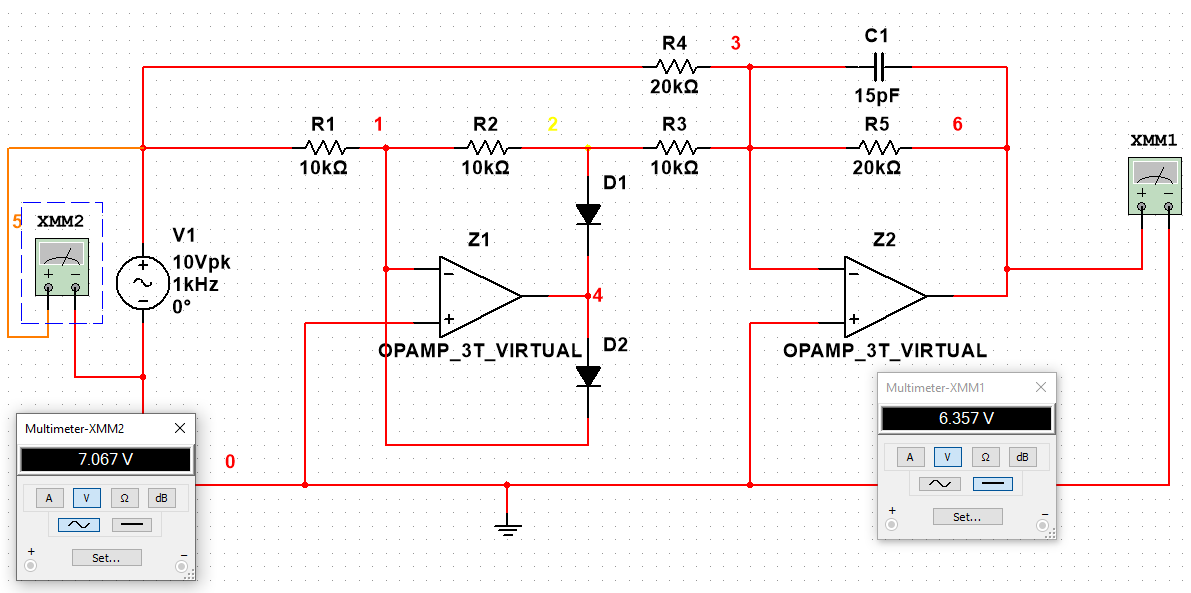
\includegraphics[width=0.8\linewidth]{schema_overeni.png}
    \caption{Schéma pro ověření správnosti funkce obvodu}
    \label{fig:schema_overeni}
\end{figure}

Na zapojení dle schématu \ref{fig:schema_overeni} byl na vstup obvodu připojen
harmonický průběh $u_1(t) = 10 \sin \left(2000\pi t\right) [\si{\volt}]$.
Na výstupu obvodu bylo multimetrem změřno stejnosměrné napětí $U_2 = 6,357 \si{\volt}$.
Platí $1,11 \cdot  U_2 = 7,057 \si{\volt}$, kde $k = 1,11$ je činitel tvaru, což odpovídá efektivní hodnotě naměřené 
na vstupu s drobnou chybou přibližně 10 \si{\milli\volt}.

\newpage
\section{Časové průběhy napětí}

\begin{figure}[h!]
    \centering
    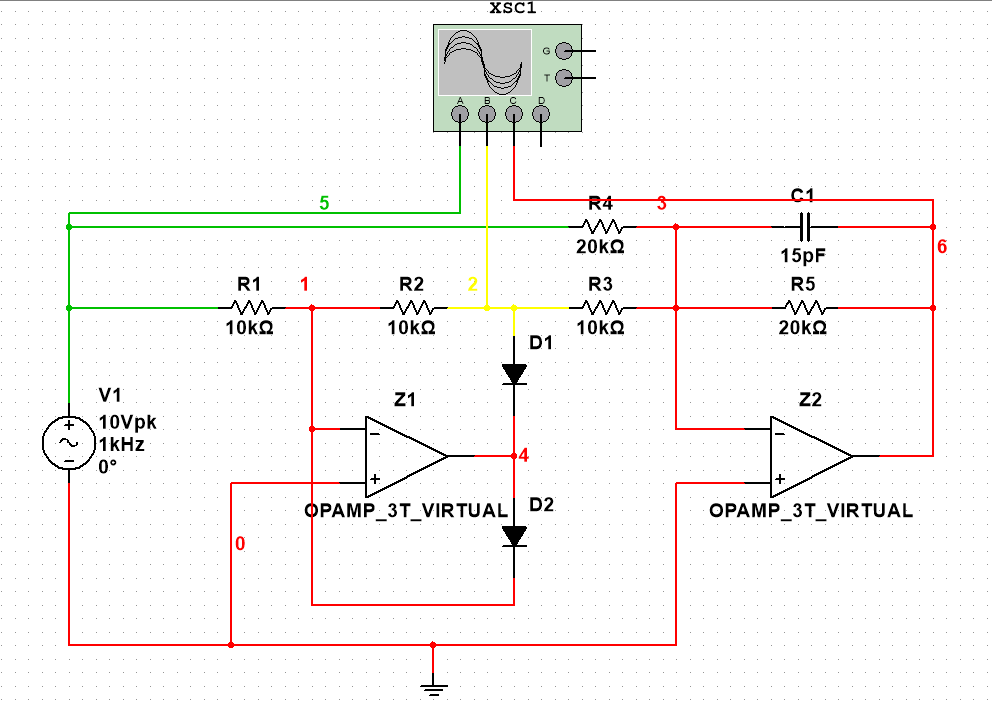
\includegraphics[width=0.8\linewidth]{prubehy_schema.png}
    \caption{Schéma pro zachycení časových průběhů napětí v různých uzlech obovodu}
    \label{fig:schema_prubehy}
\end{figure}

Zapojením osciloskopu dle schématu \ref{fig:schema_prubehy} bylo možné zachytit průběhy vykreslené
na obrázku \ref{fig:prubehy}. Zelený průběh je vstupní harmonický signál s amplitudou 10 V a frekvencí 1 kHz.
Žlutě je průběh na výstupu jednocestného usměrňovače (uzel 2), zatímco červený průběh je výstup celého 
dvoucestného usměrňovače (uzel 6). Výstup dvoucestného usměrňovače je skutečně absolutní hodnotou vstupního napětí.

\begin{figure}[h!]
    \centering
    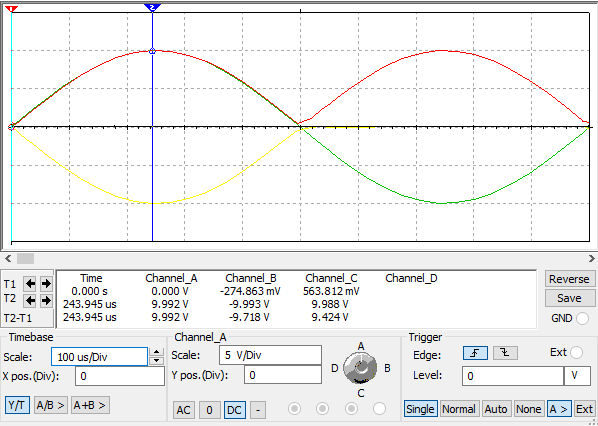
\includegraphics[width=0.8\linewidth]{prubehy_usmernovacu.png}
    \caption{Časové průběhy na výstupu jednotlivých stupňů usměrňovače}
    \label{fig:prubehy}
\end{figure}


\section{Statická převodní charakteristika}

Pomocí funkce \text{DC sweep} a byla vykreslena převodní charakteristika na obrázku \ref{fig:prevod_char}.
Žlutá charakteristika je napětí v uzlu 2, které přísluší k jednocestnému usměrňovači kolem Z1.
Červený průběh je napětí v uzlu 6, což je výstup invertujícího sumátoru, tedy výstup celého dvoucestného zesilovače.

Kurzory jsou vyznačeny dva body: na jednom je na vstupu připojeno napětí blízké 0 \si{\volt}, z čehož lze odečíst
chyby nul obou stupňů. V případě jednocestného usměrňovače je to přibližně 1,3 \si{\milli\volt}, zatímco v případě dvoucestného
je to pouhých 20 \si{\micro\volt}.
Druhý bod je umístěn poblíž vstupního napětí 5 \si{\volt}, oba stupně obvodu mají chybu menší než 20 \si{\milli\volt}
od ideální převodní charakteristiky.


\begin{figure}[h!]
    \centering
    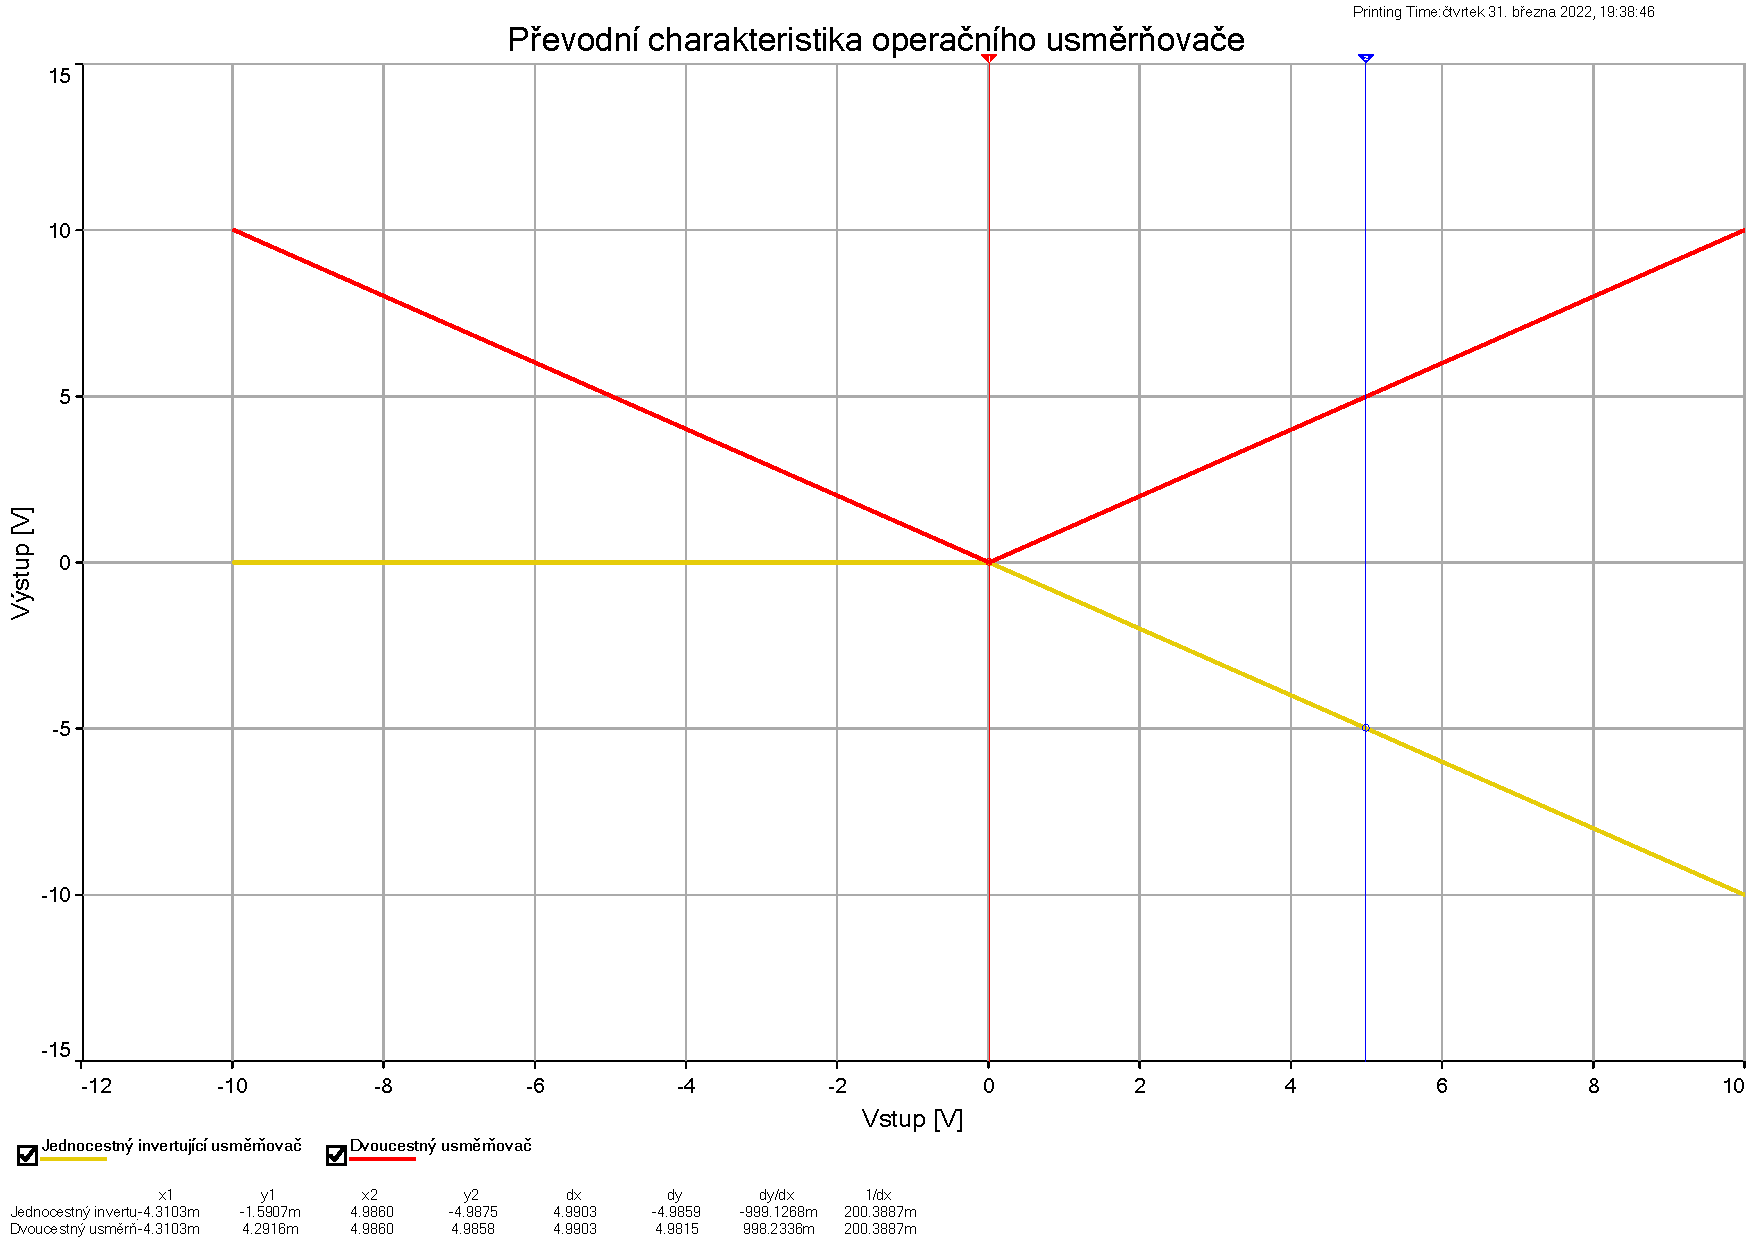
\includegraphics[width=0.55\linewidth]{prevod_char.pdf}
    \caption{Převodní charakteristika jednotlivých částí obvodu}
    \label{fig:prevod_char}
\end{figure}



\section{Frekvenční charakteristika}

Na obrázku \ref{fig:bode} je frekvenční charakteristika dvoucestného operačního usměrňovače.
Pro frekvence do cca 1 \si{\kilo\hertz} je přenos jednotkový, následuje malé převýšení před mezním kmitočtem,
který je na frekvenci $f_m = 495 \si{\kilo\hertz}$.


\begin{figure}[h!]
    \centering
    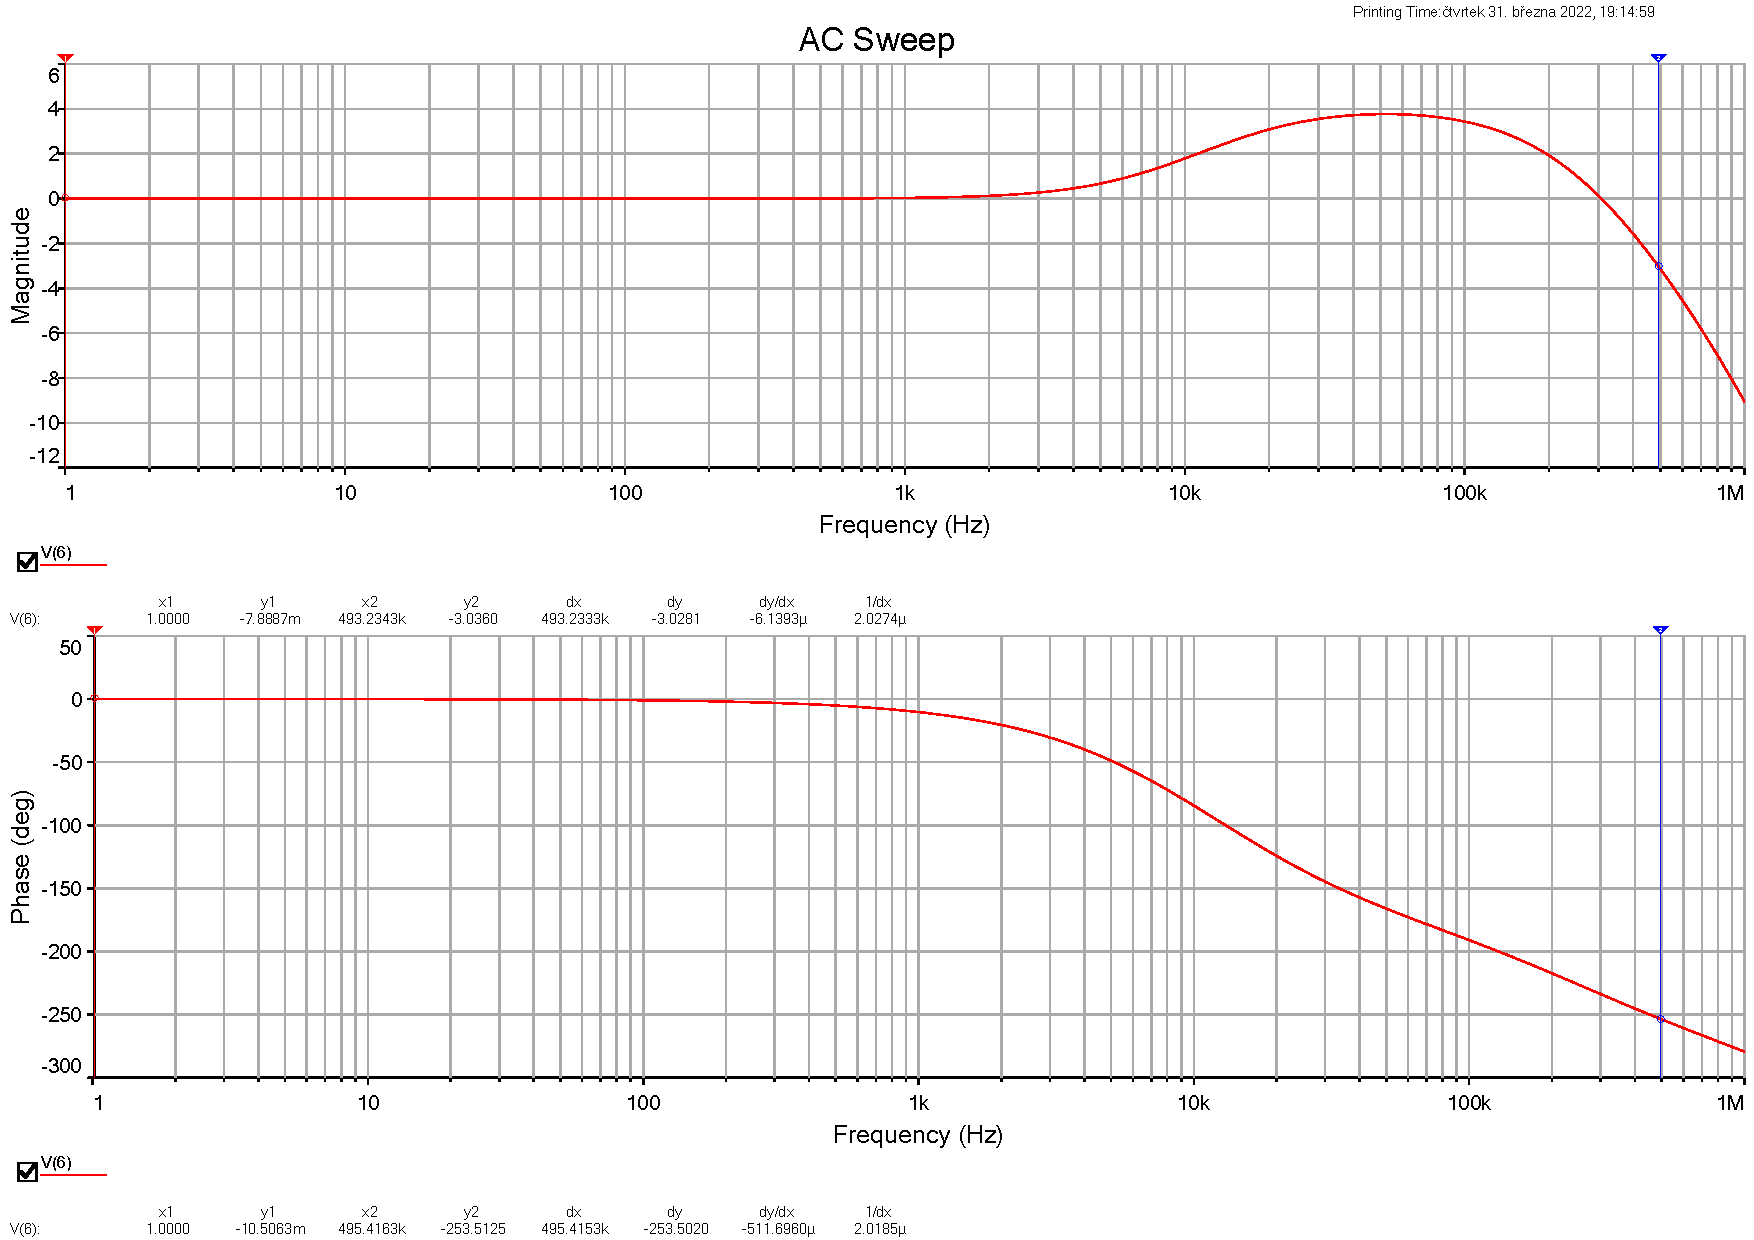
\includegraphics[width=0.8\linewidth]{frek_char.pdf}
    \caption{Frekvenční charakteristika operačního usměrňovače}
    \label{fig:bode}
\end{figure}

\section{Dynamická převodní charakteristika}

Na vstup obvodu bylo připojeno několik různých napětí při frekvenci 1 \si{\kilo\hertz}.
Změřené napětí na výstupu je uvedené v tabulce \ref{tab:prevod_char}.

\begin{table}
    \centering\begin{tabular}{c|c|c|c}
        amplituda vstupu $U_1$ [\si{\volt}] & přesné $U_{1_\text{RMS}}$ [\si{\volt}] & změřená aritmetická střední hodnota $U_{1_\text{sar}}$ [\si{\volt}] & vypočtené $U_{1_\text{RMS}}$ [\si{\volt}] \\ \hline
        1 & 0,706 & 0,6347 & 0.705 \\
        2 & 1,413 & 1,271 & 1.410 \\
        3 & 2,12 & 1,907 & 2,117 \\
        4 & 2,827 & 2,544 & 2,824 \\
        5 & 3,534 & 3,179 & 3,529 \\
        6 & 4,24 & 3,815 & 4,235 \\
        7 & 4,947 & 4,451 & 4,941 \\
        8 & 5,654 & 5,085 & 5,644 \\
        9 & 6,361 & 5,722 & 6,351 \\
        10 & 7,067 & 6,358 & 7,057
    \end{tabular}
    \caption{Převodní charakteristika operačního usměrňovače pro střídavé vstupní napětí}
    \label{tab:prevod_char}
\end{table}

Velikost absolutní chyby převodní charakteristiky v závislosti na velikosti vstupního signálu je vykreslena na grafu \ref{fig:chyba}

\begin{figure}[h!]
    \centering
    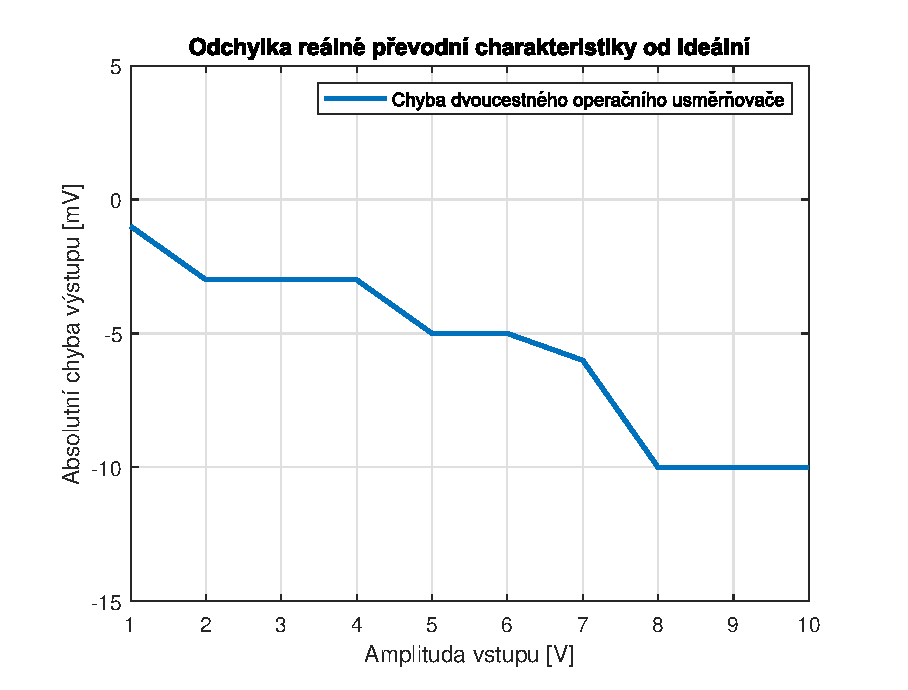
\includegraphics[width=0.8\linewidth]{chyba_prevodu.eps}
    \caption{Absolutní chyba dvoucestného operačního zesilovače}
    \label{fig:chyba}
\end{figure}


\end{document}

